\chapter{Background}

\section{Instruction Set architecture}

Instruction Set Architecture (ISA) defines the set of instructions and the registers on which they operate. Normally, the instruction operands are read from the registers and the execution result is stored there. ISA serves as an interface between software and actual hardware microarchitecture which implements the ISA. 

\TODO{what is ISA-state, instructions-granularity. ISA-level reigsters, mapping to real regs}

\section{Microarchitecture}

ISA defines binary format of instructions which are stored in memory and accessed by the processor through cache mechanisms, usually, fixed length instructions are used, while cariable-length also exist. (\TODO{add examples}). Processor is a cycled device that performs fetching instructions from memory and their subsequent execution, we call the microarchitectural state the state of all hardware registers of the processor. Unlike in ISA, states are defined at clock-cycle granularity, so an instruction takes several clock-cycles to finish. Different optimizations, such as pipelining, multiscalar execution, out-of-order execution and brach predictors (speculative execution).

\subsection{Processor Pipeline Stages}

Each instruction needs several microopererations to be executed: first, the instruction is to be loaded from memory, the operands need to be loaded from the registry. After that the instruction is executed during several cycles depending on its type (for example, multiplication is longer than addition). Due to the fact of isolation of those micropererations, it is possible to execute several instructions simultaneously: when instructions free its stage, next instruction enters it. This optimization, called pipelining, allows to increase the throughput of the processor.

\TODO{Is the word "microopererations" correct here?}

Several decompositions can exist for modern processors. Here we describe the 5 stages that can found in any processor and some of which may be further decomposed in more sophisticated architectures.

\subsubsection{Instruction Fetch (IF)}

As it was said before, the program instructions reside in global memory. This means that instructions access needs to be performed through memory hierarchy using program counter (PC) address. Often, a special instruction cache exists for accessing the program. IF stage is also responsible for updating PC to read the new instruction.

\subsubsection{Instruction Decode (ID)}

Once the instruction is fetched from memory, it exists in a processor in a packed binary format. This encoding includes the type of instruction as well as the registers it operates with. Decode stage loads the actual values from Physical Registry File (PRF) and propagates them to downstream pipeline stages. Sometimes the value can be obtained through bypass network before it appears in PRF.

\subsubsection{Execute (EX)}

EX stage computes the result of the operation. Several components may be responsible for performing different types of operations (for instance, different components for addition and multiplication). In this case IF stage emits control signals that determine the data path.

In case of memory or jump instruction the address is calculated.

The result of the computation is directly available to the ID stage via bypass network.

\subsubsection{Access Memory (MEM)}

This stage performs access to the global memory through memory hierarchy. If instruction is not a memory instruction, this stage is skipped.

\subsubsection{Commit (COM)}

The purpose of the last stage is to write the result of the instruction to PRF. Only after this the result is visible from ISA-state perspective.

\subsection{Restrictions}

The structure of the program imposes limitations on execution. Instruction may block each other thus stalling the pipeline. 

\subsubsection{Data Hazards}

There exist three types of register dependencies that may cause pipeline stall.

\textbf{Read-After-Write (RAW)} dependencies, also called as true data dependencies, arise when to perform one operation, the result of the other must be obtained. For example expression $(1 + 2 * 3)$ requires $(2 * 3)$ be calculated first, thus creating \textit{RAW}-dependency between multiplication and addition operations.

\textbf{Write-After-Write (WAW)} dependency happens when two instructions are writing to the same ISA-level register. The two writes must happen is instruction order.

\textbf{Write-after-Read (WAR)} dependency exists when the younger instruction aims at writing a value in the register which is to be read by an older instruction.

RAW-hazards are inevitable in any architecture. WAW and WAR dependencies do not exist in the model we described so far, by must be resolved in out-of-order pipeline.

\subsubsection{Control Hazards}

Fetching next instruction is possible only if the address of it is known. In case of branches, the next instruction address is not known until the branch outcome is calculated in execute stage.

Therefore, the so-called bubbles (which denote the absence of operation) are introduced into the pipeline.

\begin{figure}
    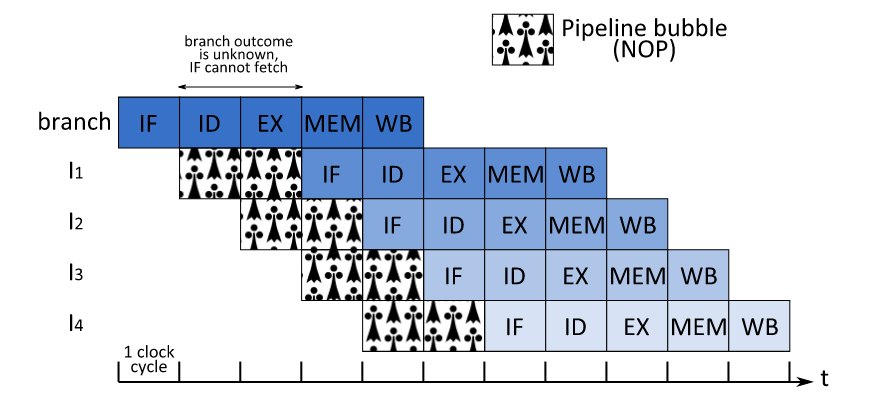
\includegraphics[width=\textwidth]{figures/pipeline-bubbles.png}
    \caption{Example of control hazard: the pipeline is stalled until branch finished the execution (from \cite{perais_increasing_2016})}
    \label{fig:bubbles}
\end{figure}

\subsection{Multiscalar Execution}

Instead of fetching instructions one by one, it is possible to fetch several ones in the same time. This also means that other stages are also multiplied to accommodate all fetched instructions. Since neighbor instructions may be independent this can significantly increase the performance. However, duplicating each stage is costly, while it is relatively easy for IF, ID and COM, execution and accessing memory is much harder to duplicate.

\subsection{Out-of-Order (OoO) Pipeline}

Despite the fact that the instructions are to be processed in program order, many of them are in fact independent. This means that the order of execution can be chosen based on instruction dependencies rather than their order in initial program. Notice that the pipeline is often stalled by the execution of long instructions (\TODO{refer visual example}). The key idea is that while one instruction is being executed on one functional unit (FU), the other, independent of this one can be executed on the other FU. 

In this approach we divide the pipeline into in-order and out-of-order parts. In-order consists of IF, ID and COM stages while out-of-order includes execution and memory accesses. This allows to achieve a consistent ISA-stage due to in-order fetch a commit. 

Different mechanisms exist to synchronize out-of-order execution. Here we introduce reservation stations (RS) and reorder buffer (ROB) - the additional pipeline stages.

Reservation station is a queue before the functional unit, each FU is equipped with its own RS. Once the instruction is decoded it is forwarded to FU based on its type, but if FU is busy, the instruction is put instead into the corresponding RS. Subsequently, the FU is taking the instructions both from ID and RS based on the scheduling policy.

ROB is a FIFO queue that insures the order in which instructions should be committed. Each time, the instruction enters out-of-order part (RS or FU) it is also appended to the front of ROB. After being executed, the instruction is tagged as ready in the ROB. The COM stage commits only the last instruction (or several if multiscalar) from the ROB if it is ready, thus ensuring commit in program order.

\TODO{Image}

\subsection{Branch Prediction}

IF stage is responsible for fetching the next instruction in the program. However, when conditional jump instruction is fetched the next read address is undefined until the outcome of condition is calculated. The straightforward approach is to stall the pipeline, introducing so-called bubbles (no operation).

The more advanced approach consists of fetching a new instruction anyway, the address of which is guessed by branch prediction mechanism, discussed further. Such instructions are called speculative and are not committed until branch decision is taken. In case of incorrect prediction speculative instruction are flushed from the pipeline. 

\section{Branch Predictor Implementations}

\subsection{Static Branch Predictors}

Static branch prediction relies on information known at compile time. Some well-known static branch predictors are:

\begin{itemize}
    \item Always Not Taken
    \item Always Taken
    \item Backward Taken, Forward Not Taken
\end{itemize}

\TODO{add details}

\subsection{Dynamic Branch Predictors}

Dynamic Branch Predictors rely on information retrieved from execution and are usually based on previous branch outcomes. The usage of dynamic branch predictors requires additional hardware components which are discussed below.

\textbf{Pattern History Table (PHT)} is used to store information about each branch. It can be a bit denoting whether the branch was taken last time, or a more complex data. PHT is usually indexed by the lower bits of branch instruction address.

\textbf{Branch Target Buffer (BTB)} stores the destinations of previously computed branch. When starting speculative execution, values from BTB are used.

\textbf{Return Stack Buffer (RSB)} is used to predict the outcome of \textit{ret} instructions.

\subsubsection{One-Bit Predictor}

The one-bit predictor is the simplest type of dynamic branch predictor. It uses PHT indexed by lower bits of address where one-bit value encodes the last branch outcome. Such a simple predictor is efficient when branch decision is not often changed throughout execution. For example, loop conditions are mispredicted only twice by this type of predictor: on the first and the last iterations of the loop.

However, more complex patterns diminish the efficiency of one-bit predictor. For instance, if branch outcome changes each time, the predictor accuracy is zero.

\subsubsection{Two-Bit Predictor}

The two-bit predictor uses the same idea of PHT-indexing, but instead of storing just the outcome of previous branch, it has 4-state automaton encoded by 2 bits. The states are STRONG-TAKEN, WEAK-TAKEN, WEAK-NTAKEN and STRONG-NTAKEN. Picture \TODO{} shows the transitions between the states.

\begin{figure}
    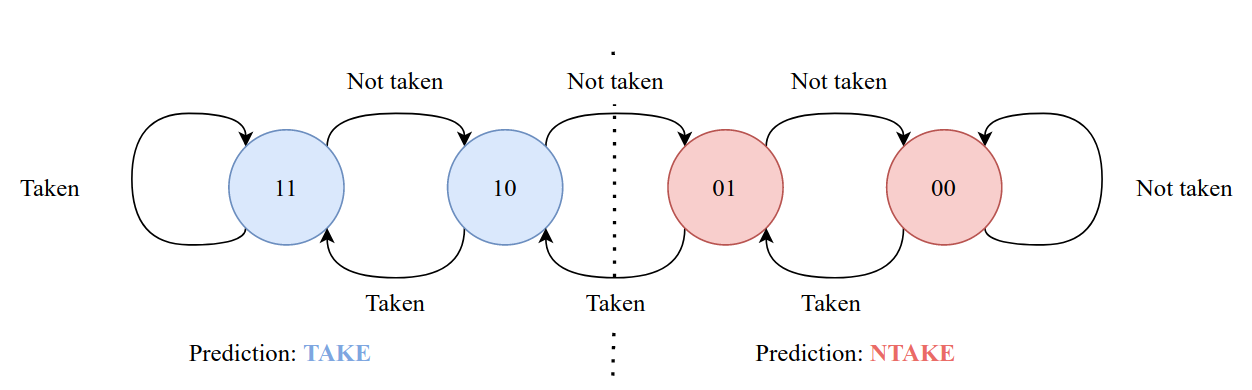
\includegraphics[width=\textwidth]{figures/two-bit-counter.png}
    \label{fig:two-bit-counter}
    \caption{Two-bit predictor state machine (from \cite{mahling_reverse_2023})}
\end{figure}

\TODO{why better than 1-bit}

\TODO{other types. which are used in critical systems?}


\section{WCET Analysis}

In critical systems such as \TODO{examples} it is important that the tasks executed on the hardware meet their deadlines. This is ensured by worst execution time (WCET) analysis. It takes the pair of the program and the dedicated hardware and aims at giving an upper-bound on execution time. 

\TODO{stages of WCET-analysis}

\section{Timing Anomalies}

Phase ordering is a major chellange in WCET-analysis. Most of analysis steps require information from each other (\TODO{examples}), so it is not always possible to order them. 

Nevertheless, most architectures are not composable and contain so-called timing anomalies (TA). Intuitively, TA happens when local worst cases do not constitute a global worst case. TA is observed on the pair of execution traces where the initial hardware state differs, and the instruction sequences are identical. Different cache states can be the source of variation in timing behavior due to miss in one trace and hit in another one.

Figure \ref{fig:TA1} shows the example of such an anomaly. Here, the assembly sequence consists of 4 instructions ($A,B,C,D$) with data dependencies $A \rightarrow B$ and $C \rightarrow D$. Figure \ref{fig:TA1-trace} represents the pair of traces ($\alpha, \beta$) derived from execution of the given program. There is a variation in latency of instruction $A$ ($1$ in $\alpha$ and $2$ in $\beta$). In trace $\alpha$  the variation is favorable, but the total execution time is also higher in this trace which signals an anomaly.

\begin{figure}[htbp]
    \centering
    \begin{subfigure}[t]{0.3\textwidth}
        \centering
        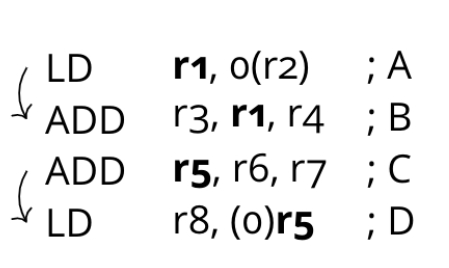
\includegraphics[width=\textwidth]{figures/first-TA-ex-input.png}
        \caption{Inpus assembly sequence}
        \label{fig:TA1-code}
    \end{subfigure}
    \hfill
    \begin{subfigure}[t]{0.55\textwidth}
        \centering
        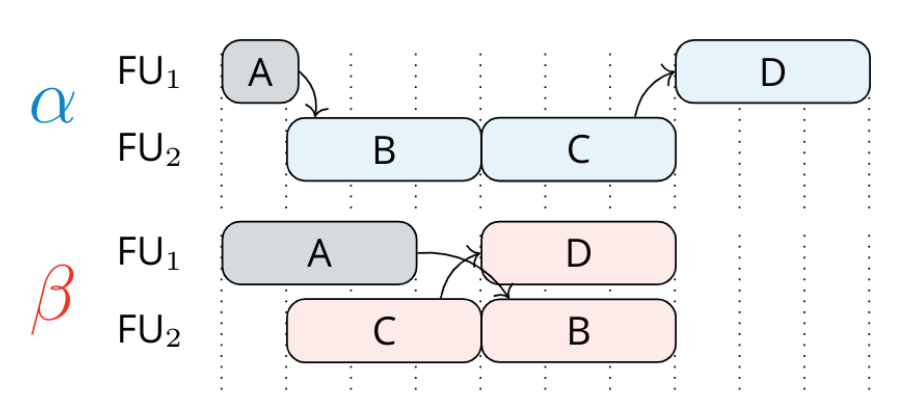
\includegraphics[width=\textwidth]{figures/first-TA-ex-trace.png}
        \caption{Scheduling on functional units comparison}
        \label{fig:TA1-trace}
    \end{subfigure}
    \caption{TA caused by variation in latency of instruction \textit{A} (from \cite{binder_definitions_2022})}
    \label{fig:TA1}
\end{figure}


non-composable architectures

amplification and counter-intuitive TAs